\documentclass[11pt]{article}
\usepackage{amssymb,amssymb,amsmath,graphicx}
\usepackage{hyperref}


\let\hat\widehat
\let\tilde\widetilde
%\usepackage[dvips]{color}
\setlength{\oddsidemargin}{0in}
\setlength{\evensidemargin}{0in}
\setlength{\textwidth}{6.3in}
\setlength{\topmargin}{0in}
\setlength{\headsep}{0in}
\setlength{\textheight}{8.5in}
\renewcommand{\baselinestretch}{1} % changes spacing.
\renewcommand{\arraystretch}{1.5}
\renewcommand{\tabcolsep}{.15in}

\flushbottom

\begin{document}
\begin{center}
{\bf ISyE 6416: Computational Statistics}\\
{\bf Homework 5 \\ (100 points total. )}
\end{center}


\vspace{.2in} \noindent This homework is due on {\bf April 6, 2020}. 

\vspace{.05in} \noindent $\bullet$ Please write your team member's name if you collaborate.

\vspace{.20in}

\begin{enumerate}







\item {\bf Nonlinear regression using spline.} (40 points.)

The coefficient of thermal expansion $y$ changes with temperature $x$. An experiment to relate $y$ to $x$ was done. Temperature was measured in degrees Kelvin. (The Kelvin temperature is the Celcius temperature plus 273.15). The raw data file is \textsf{copper-new.txt} 

\begin{figure}[h!]
\begin{center}
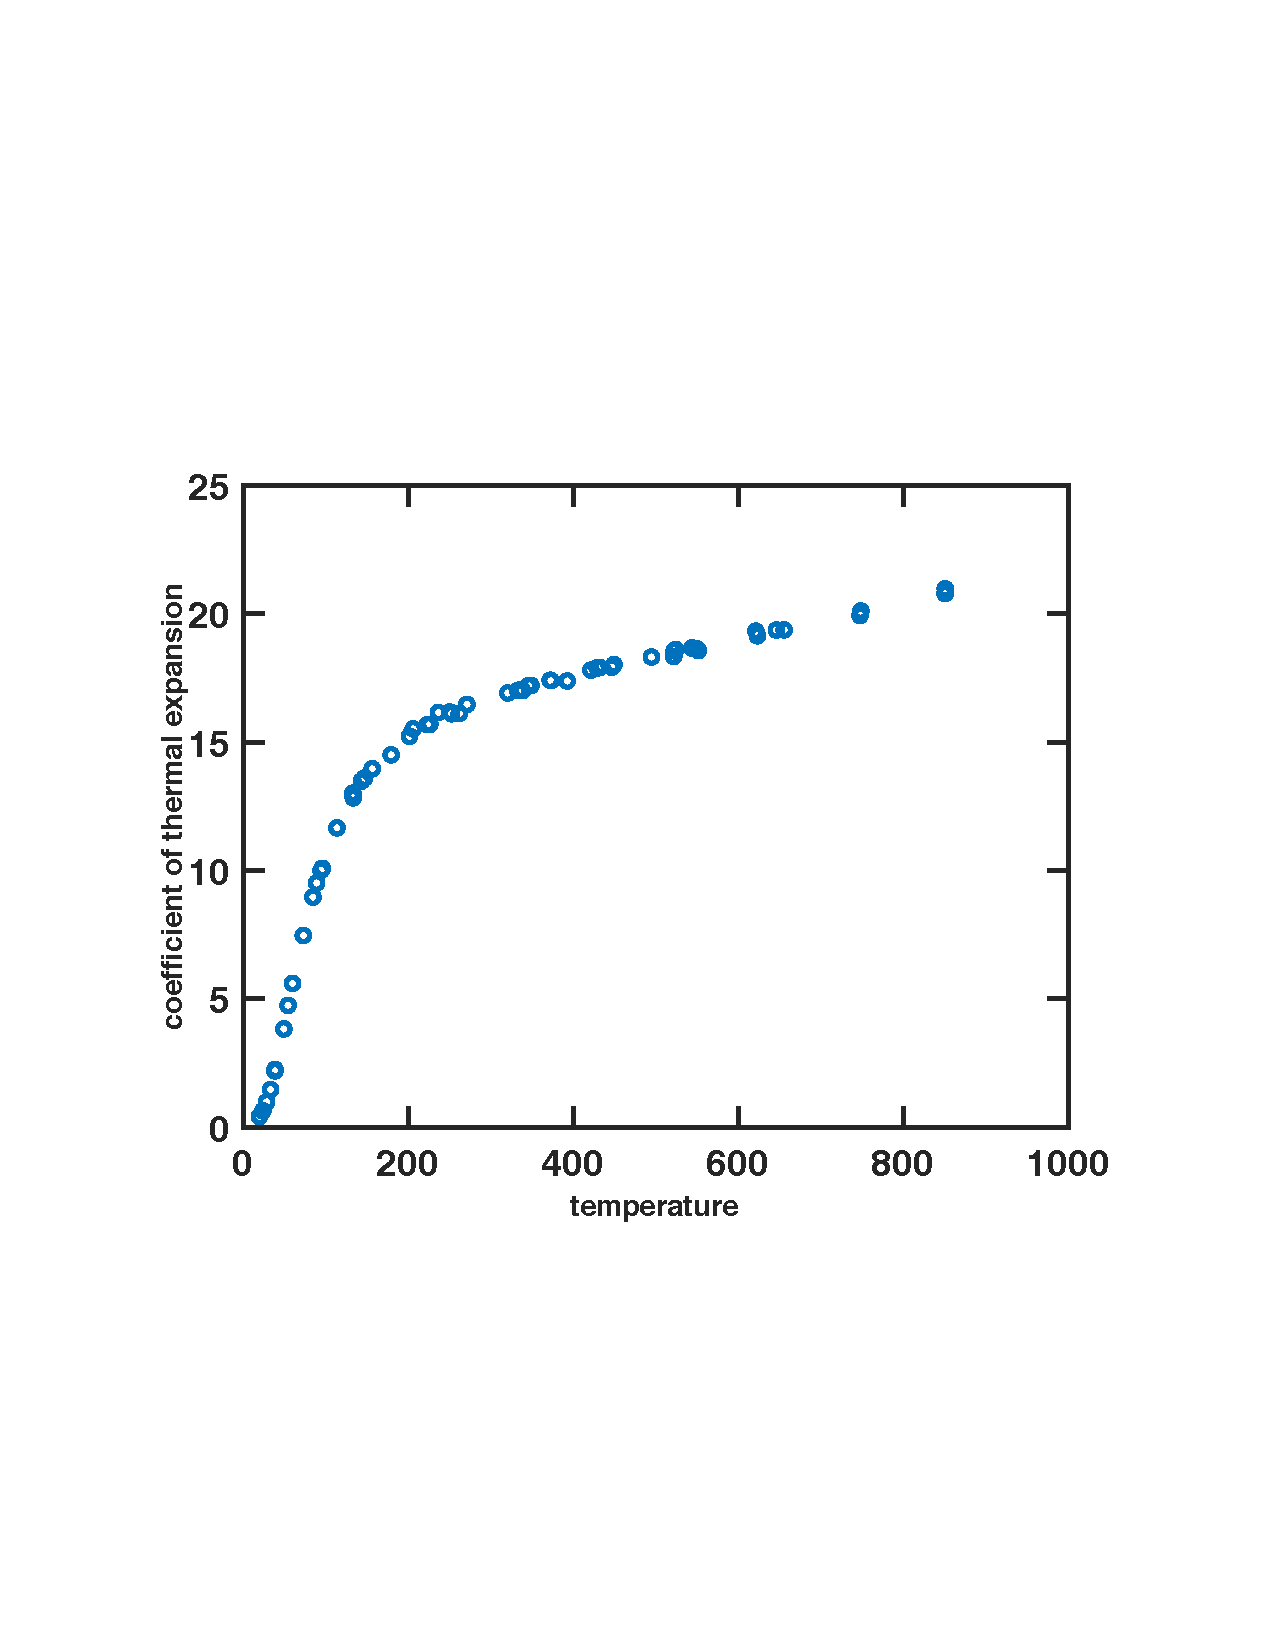
\includegraphics[width = 0.8\textwidth]{t_c}
\end{center}
\end{figure}

\begin{enumerate}

\item Perform linear regression on the data. Report the fitted model and the fitting error.
\item Perform nonlinear regression with spline function (i.e., using all data points). Use GCV for find $\lambda$. Report the fitting error. 
\item Predict the coefficient at 400 degree Kelvin.
%\item What is an upper bound for the prediction error at this 400 degree point? 
\end{enumerate}

\item {\bf PCA for face recognition.} (30 points.)

\begin{enumerate}
\item Perform data analysis on the Yale face dataset (in Canvas) for subject 14. Plot the mean face and the first 6 eigenfaces for subject 14.
\item Now use \textsf{subject14.test.gif} to perform face recognition using the following procedure. 
\end{enumerate}

For doing face recognition through PCA we proceed as follows. Given the test image, we project it using the first component to obtain the coefficient vector, and compare $|z^\intercal u_{1, i}|$, $i = 1, 2$, where $u_{1, i}$ is the first dominant component for $i$th person. Are we able to recognize the person correctly using the first principle component? 

{\bf Remark:} you have to perform downsampling of the image by a factor of 4 to turn them into a lower resolution image before we do anything. See the example MATLAB code. 


\item {\bf Recommender systems.} (30 points)

Take our movie recommender systems data (which is obtained from a course survey in previous year), and perform recommendation using the following methods. Hint, when using features, expanding the categorical features using ``one-hot'' keying.

\begin{enumerate}
\item User-based collaborative filter to recommend 5 movies to each user. Try several similarity metrics, which are defined in the forms of 
\[
\mbox{sim}(u, v) = e^{-(d(u, v))^2},
\]
where \begin{enumerate}
\item (1) $d(u, v) = \ell_2$ distance of the features, i.e., if $x_u$ is the feature vector of the first movie, and  $x_v$ is the feature vector of the second movie, then $d(u, v) = \|x_u - x_v\|_2$. 
\item (2) $d(u, v) = \ell_1$ distance of the features, i.e.,  $d(u, v) = \|x_u - x_v\|_1$; 
\item (3) $d(u, v) = $Hamming distance of the features, i.e., $d(u, v) = \|x_u - x_v\|_0$; 
\end{enumerate}
\item Item-based recommendation to recommend 5 movies to each user. try using the above three metrics respectively. 
\item Using matrix completion algorithm based on soft-impute (R package \url{https://cran.r-project.org/web/packages/softImpute/softImpute.pdf})\footnote{More reference here \url{https://web.stanford.edu/~hastie/swData/softImpute/vignette.html}} to fill out missing entries to recommend 5 movies to each user.
\end{enumerate}

Report all of the three findings in an excel spread sheet (with 3 tabs for each of methods), and each row is in the format of \textsf{(name,  recommended movie 1, score of the recommended movie 1, ..., recommended movie 5, score of the recommended movie 5}).


\end{enumerate}


\end{document}




































